%!TEX root = ../TechnischerEntwurf.tex

\chapter{Datenmodell}

Das folgende Kapitel beschreibt die Datensätze, welche der SQL-Alchemist dauerhaft oder teilweise auch nur temporär abspeichert.
Dazu werden zuerst einige Erl\"auterungen zu den einzelnen Beziehungen angegeben und zum Ende des Kapitels ist ein Klassen-Diagramm zur Veranschaulichung dieses Sachverhaltes abgebildet.


\section{Erläuterung}


\begin{entity}{10}{Avatar}
\begin{center}
	\begin{longtable}{|m{4cm}|m{2,5cm}|m{4,5cm}|m{3,5cm}|}
 	 \hline
 	 \textbf{Beziehung} & \textbf{Kardinalität} &  \textbf{Erwartete Datenmenge} & \textbf{Beschreibung} \\
  	\hline
  	Profile & 0 ... *   & Min: 1kB, Max: 100kB & Der Avatar wird vom Profil als Erkennungsmerkmal und Spielfigur verwendet.\\
  	  	\hline
  	Profile\_Avatar & 1 ... *   & - & Verweis auf alle vom Nutzer gekauften Avatare.\\
	  \hline
	\end{longtable}
\end{center}
Die Entitäten vom Typ \glqq Avatar\grqq~beschreiben die verschiedenen vom Spiel zur Verfügung gestellten Spielfiguren. Diese werden sowohl im Minispiel als auch als Erkennungsmerkmal der Profile der Nutzer verwendet.
In der Datenbank werden unter anderem die zugehörigen Eigenschaften, sowie die Darstellungsmerkmale gespeichert.
\textbf{Hinweis:} In der Relation Profile\_Avatar sind die Avatare mit den Profilen verknüpft, das Profil verfügt jedoch zusätzlich über das Attribut \glqq Avatar\grqq. Der im Profil gespeicherte Avatar ist dabei der aktuell verwendete.
\end{entity}


\newpage
\begin{entity}{20}{Bag}
\begin{center}
	\begin{longtable}{|m{4cm}|m{2,5cm}|m{4,5cm}|m{3,5cm}|}
 	 \hline
 	 \textbf{Beziehung} & \textbf{Kardinalität} &  \textbf{Erwartete Datenmenge} & \textbf{Beschreibung} \\
  	\hline
  	Potion & 1  & Min: 1 kB, Max: 16 kB & In Bagslots werden die bereits gesammelten Tränke gespeichert.\\
	  \hline
  	Profile & 1  & Min: 1 kB, Max: 100 kB & Ein Bagslot gehört einem Profil.\\
	  \hline
	\end{longtable}
\end{center}
Bei den Entitäten des Typs \glqq Bag\grqq~handelt es sich um die einzelnen Plätze innerhalb des Inventars der Nutzer, in denen alle hergestellten Tränke abgelegt werden. Dabei nimmt jeder Slot genau einen Trank auf. \\\\\
\end{entity}


\begin{entity}{30}{Challenge}
\begin{center}
	\begin{longtable}{|m{4cm}|m{2,5cm}|m{4,5cm}|m{3,5cm}|}
 	 \hline
 	 \textbf{Beziehung} & \textbf{Kardinalität} &  \textbf{Erwartete Datenmenge} & \textbf{Beschreibung} \\
  	\hline
  	Map\_In\_Challenge & 0 ... *  & - & Eine Challenge kann mit mehreren Maps verknüpft sein.\\
	  \hline
  	Text\_In\_Challenge & 0 ... *  & - & Story-Texte können Challenges zugeordnet werden, um diese in den Kontext der Handlung einzubinden. \\
	  \hline
	Task\_In\_Challenge & 1 ... * & 8 B & Eine Challenge besteht aus mindestens einer Aufgabe.\\
	  \hline
	\end{longtable}
\end{center}
Die \glqq Challenge\grqq-Objekte beschreiben die Aufgabenpakete, welche zum Beispiel im Laufe der Story oder als Hausaufgaben an die Nutzer gestellt werden. Jedes dieser Pakete besteht aus verschiedenen Aufgaben. Als Attribute werden alle Informationen, die zur Beschreibung eines solchen Paketes benötigt werden in der Datenbank gespeichert.\\\\\\\
\end{entity}

\begin{entity}{40}{Map}
\begin{center}
	\begin{longtable}{|m{4cm}|m{2,5cm}|m{4,5cm}|m{3,5cm}|}
 	 \hline
 	 \textbf{Beziehung} & \textbf{Kardinalität} &  \textbf{Erwartete Datenmenge} & \textbf{Beschreibung} \\
  	\hline
  	Map\_In\_Challenge & 0 ... *   & - & Eine Map kann in mehreren Challenges verwendet werden.\\
	  \hline
	\end{longtable}
\end{center}
Bei den \glqq Map\grqq-Entitäten handelt es sich um die verschiedenen Levels, aus denen das Minispiel besteht. \\\\\\\
\end{entity}

\begin{entity}{50}{Map\_In\_Challenge}
\begin{center}
	\begin{longtable}{|m{4cm}|m{2,5cm}|m{4,5cm}|m{3,5cm}|}
 	 \hline
 	 \textbf{Beziehung} & \textbf{Kardinalität} &  \textbf{Erwartete Datenmenge} & \textbf{Beschreibung} \\
  	\hline
  	Challenge & 1  & ca. 28 byte & Verweis auf die Challenge\\
	  \hline
  	Map & 1 & Min: 512 byte, Max: 16 kB & Verweis auf die Map\\
	  \hline
	\end{longtable}
\end{center}
In diesen Objekten werden die Beziehungen der \glqq Maps\grqq~und der \glqq Challenges\grqq~festgehalten. Dies umfasst, welche Level des Minispiels für die Lösung bestimmter Aufgabenpakete abgeschlossen werden müssen und in welcher Reihenfolge diese auftreten. \\\
\end{entity}

\begin{entity}{60}{Potion}
\begin{center}
	\begin{longtable}{|m{4cm}|m{2,5cm}|m{4,5cm}|m{3,5cm}|}
 	 \hline
 	 \textbf{Beziehung} & \textbf{Kardinalität} &  \textbf{Erwartete Datenmenge} & \textbf{Beschreibung} \\
  	\hline
  	Bag & 0 ... *  & 16 byte & Die Potion wird in einem Bagslot abgelegt.\\
	  \hline
  	Scroll & 1  & Min: 50 byte, Max: 500 byte & Die Potion ist einer Scroll zugeordnet. \\
	  \hline
  	Task & 1 ... *  & Min: 300 byte, Max: 5 kByte & Zum Erzeugen der Potion muss eine Aufgabe gelöst werden.\\
	  \hline
	\end{longtable}
\end{center}
Die \glqq Potion\grqq-Entitäten beschreiben die Tränke, welche die Spieler im Laufe des Spiels herstellen. Dazu werden die Auswirkungen der Tränke als Attribute gespeichert. \\\\\\\
\end{entity}

\begin{entity}{70}{Profile}
\begin{center}
	\begin{longtable}{|m{4cm}|m{2,5cm}|m{4,5cm}|m{3,5cm}|}
 	 \hline
 	 \textbf{Beziehung} & \textbf{Kardinalität} &  \textbf{Erwartete Datenmenge} & \textbf{Beschreibung} \\
  	\hline
  			Avatar & 1 & Min: 500 byte, Max: 32 kByte & Jedes Profil besitzt einen Avatar, der dieses repräsentiert.\\
	  \hline
	    	Bag & 0 ... * & 16 byte & Bagslots, die dem Profil gehören.\\
	  \hline
  			Profile\_Avatar & 0 ... *  & - & Dem Profil zur Verfügung stehende Avatare.\\
	  \hline
	    	Comment\_Task & 0 ... * & - & In dieser Relation wird auf die vom Nutzer kommentierten Aufgaben verwiesen. \\
	  \hline
	    	Rate\_Task & 0 ... * & - & In dieser Relation wird auf die vom Nutzer bewerteten Aufgaben verwiesen.\\
	  \hline
	    	Profile\_Scroll & 0 ... * & 8 byte & Das Profil sammelt Schriftrollen in der Scrollcollection.\\
	  \hline
	    	Profile\_Shop\_Item & 0 ... * & 8byte & Relation mit gekauften Items im Shop.\\
	  \hline 
	    	Solve\_Task & 0 ... * & 20 byte & Tasks, zu denen der Nutzer Zugang hat.\\
	  \hline
  	  		User & 1  & Min: 250 byte, Max: 150 kByte &  Jedes Profil gehört einem Nutzer.\\
	  \hline
	\end{longtable}
\end{center}
Die Entitäten des Typs \glqq Profile\grqq~stellen die zentrale Verwaltungsstelle der Nutzer dar. Über diese wird der Fortschritt der Spieler abgewickelt, deren Einstellungen gespeichert und die Eigenschaften der Spielfiguren festgehalten. 
\end{entity}

\newpage
\begin{entity}{80}{Profile\_Avatar}
\begin{center}
	\begin{longtable}{|m{4cm}|m{2,5cm}|m{4,5cm}|m{3,5cm}|}
 	 \hline
 	 \textbf{Beziehung} & \textbf{Kardinalität} &  \textbf{Erwartete Datenmenge} & \textbf{Beschreibung} \\
  	\hline
	Avatar & 1  & Min: 500 byte, Max: 32 kByte & Verweis auf ein Avatar\\
	  \hline
  	Profile & 1  & Min: 1 kByte, Max: 100 kByte & Verweis auf ein Profil\\
	  \hline
	\end{longtable}
\end{center}
Diese Entitäten halten die durch ein Profil gekauften Avatare fest und speichert dazu wann die Transaktion durchgeführt wurde.\\\\\\\
\end{entity}

\begin{entity}{90}{Comment\_Task}
\begin{center}
	\begin{longtable}{|m{4cm}|m{2,5cm}|m{4,5cm}|m{3,5cm}|}
 	 \hline
 	 \textbf{Beziehung} & \textbf{Kardinalität} &  \textbf{Erwartete Datenmenge} & \textbf{Beschreibung} \\
  	\hline
	Profile & 1  & Min: 1  kByte, Max: 100 kByte & Verweis auf das Profil\\
	  \hline
  	Task & 1  & Min: 300 byte, Max: 5 kByte & Verweis auf die Aufgabe\\
	  \hline
	\end{longtable}
\end{center}
Über die \glqq Comment\_Task\grqq-Objekte werden die durch die Nutzer kommentierten Aufgaben gespeichert. Als Attribut wird dazu unter anderem das jeweilige Kommentar festgehalten.\\\\\\\
\end{entity}

\begin{entity}{100}{Rate\_Task}
\begin{center}
	\begin{longtable}{|m{4cm}|m{2,5cm}|m{4,5cm}|m{3,5cm}|}
 	 \hline
 	 \textbf{Beziehung} & \textbf{Kardinalität} &  \textbf{Erwartete Datenmenge} & \textbf{Beschreibung} \\
  	\hline
	Profile & 1  & Min: 1 kByte, Max: 100 kByte & Verweis auf das Profil\\
	  \hline
  	Task & 1  & Min: 300 byte, Max: 5 kByte & Verweis auf die Aufgabe\\
	  \hline
	\end{longtable}
\end{center}
Über die \glqq Rate\_Task\grqq-Objekte werden die durch die Nutzer bewerteten Aufgaben gespeichert. Als Attribut wird dazu unter anderem die jeweilige Bewertung festgehalten.\\\\\\\
\end{entity}

\begin{entity}{110}{Profile\_Scroll}
\begin{center}
	\begin{longtable}{|m{4cm}|m{2,5cm}|m{4,5cm}|m{3,5cm}|}
 	 \hline
 	 \textbf{Beziehung} & \textbf{Kardinalität} &  \textbf{Erwartete Datenmenge} & \textbf{Beschreibung} \\
  	\hline
	Profile & 1  & Min: 1 kByte, Max: 100 kByte  & Verweis auf das Profil\\
	  \hline
  	Scroll & 1  & Min: 50 byte, Max: 500 byte & Verweis auf die Scroll\\
	  \hline
	\end{longtable}
\end{center}
Hier werden die von den Nutzern gesammelten Scrolls gespeichert.\\\\\\\
\end{entity}

\begin{entity}{120}{Profile\_Shop\_Item}
\begin{center}
	\begin{longtable}{|m{4cm}|m{2,5cm}|m{4,5cm}|m{3,5cm}|}
 	 \hline
 	 \textbf{Beziehung} & \textbf{Kardinalität} &  \textbf{Erwartete Datenmenge} & \textbf{Beschreibung} \\
  	\hline
	Profile & 1  & Min: 1 kByte, Max: 100 kbyte & Verweis auf das Profil\\
	  \hline
  	Shop\_Item & 1  & Min: 100 byte, Max: 1 kByte & Verweis auf das Shop-Item\\
	  \hline
	\end{longtable}
\end{center}
Die Entitäten des Typs \glqq Profile\_Shop\_Item\grqq~halten fest, welche Spielgegenstände die Spieler bisher bereits erworben haben.
\end{entity}

\newpage
\begin{entity}{130}{Solve\_Challenge}
\begin{center}
	\begin{longtable}{|m{4cm}|m{2,5cm}|m{4,5cm}|m{3,5cm}|}
 	 \hline
 	 \textbf{Beziehung} & \textbf{Kardinalität} &  \textbf{Erwartete Datenmenge} & \textbf{Beschreibung} \\
  	\hline
  	Challenge & 1  & ca. 28 byte & Verweis auf die Challenge\\
	  \hline
	Profile & 1  & Min: 1 kByte, Max: 100 kByte & Verweis auf das Profil\\
	  \hline
	\end{longtable}
\end{center}
Diese Objekte halten den Bearbeitungsfortschritt der Nutzer bezüglich der Aufgabenpakete fest. Es werden dabei sowohl die bereits gelösten Aufgabenpakete, als auch die noch nicht abgeschlossenen Aufgabenpakete abgespeichert.\\\\\\\
\end{entity}

\begin{entity}{140}{Solve\_Task}
\begin{center}
	\begin{longtable}{|m{4cm}|m{2,5cm}|m{4,5cm}|m{3,5cm}|}
 	 \hline
 	 \textbf{Beziehung} & \textbf{Kardinalität} &  \textbf{Erwartete Datenmenge} & \textbf{Beschreibung} \\
  	\hline
	Profile & 1  & Min: 1 kByte, Max: 100 kByte &  Verweis auf das Profil\\
	  \hline
  	Task & 1  & Min: 300 byte, Max: 5 kByte & Verweis auf die Aufgabe.\\
	  \hline
	\end{longtable}
\end{center}
Diese Entitäten sorgen für die Speicherung des Fortschritts bei der Lösung der einzelnen Aufgaben durch die verschiedenen Nutzer. Dabei werden unter anderem die benötigte Zeit, sowie das Lösungsdatum als Attribute gespeichert.
\end{entity}

\newpage
\begin{entity}{150}{Scroll}
\begin{center}
	\begin{longtable}{|m{4cm}|m{2,5cm}|m{4,5cm}|m{3,5cm}|}
 	 \hline
 	 \textbf{Beziehung} & \textbf{Kardinalität} &  \textbf{Erwartete Datenmenge} & \textbf{Beschreibung} \\
  	\hline
  	Potion & 0 .. 1  & Min: 1 kByte, Max: 16 kByte & Jede Schriftrolle schaltet eine oder keine Potion frei.\\
	  \hline
	Profile\_Scroll & 0 ... * & 8 byte & Eine gesammelte Schriftrolle wird in der Scrollcollection des Profils gespeichert.\\
	  \hline
	\end{longtable}
\end{center}
Die \glqq Scrolls\grqq~beschreiben die im Spiel verteilten Schriftrollen, welche durch die Spieler eingesammelt werden um neue Tränke oder temporäre Verbesserungen der Eigenschaften der Spielfigur (Buffs) freischalten. 
\textbf{Hinweis:} Wird durch die Scroll keine Potion freigeschaltet, erhält der Nutzer einen Buff. \\\\\\\
\end{entity}

\begin{entity}{160}{Shop\_Item}
\begin{center}
	\begin{longtable}{|m{4cm}|m{2,5cm}|m{4,5cm}|m{3,5cm}|}
 	 \hline
 	 \textbf{Beziehung} & \textbf{Kardinalität} &  \textbf{Erwartete Datenmenge} & \textbf{Beschreibung} \\
  	\hline
  	Profile\_Shop\_item & 0 ... *  & 8 byte & Relation zwischen Shop-Items und den Profilen der Nutzer, die das Shop-Item gekauft haben.\\
	  \hline
	\end{longtable}
\end{center}
Die Objekte des Typs \glqq Shop\_Item\grqq~stellen die im Shop zum Kauf zur Verfügung stehenden Gegenstände dar. Daher wird unter anderem der Kaufpreis als Attribut gespeichert.
\end{entity}

\newpage
\begin{entity}{170}{Story\_Text}
\begin{center}
	\begin{longtable}{|m{4cm}|m{2,5cm}|m{4,5cm}|m{3,5cm}|}
 	 \hline
 	 \textbf{Beziehung} & \textbf{Kardinalität} &  \textbf{Erwartete Datenmenge} & \textbf{Beschreibung} \\
  	\hline
  	Text\_In\_Challenge & 1 & - & Story-Texte beschreiben Challenges handlungsbezogen.\\
  	\hline
  	Text & 0 ... * & Min: 50 byte, Max: 500 byte & Texte beschreiben die Spielsituation.\\
	  \hline
	\end{longtable}
\end{center}
Diese Entitäten beschreiben die verschiedenen Texte, welche in der Story aufgerufen werden. Dazu werden die Bedingungen, welche erfüllt sein müssen um den Text aufzurufen, sowie die Reihenfolge, in der diese auftreten und deren Inhalt abgespeichert. \\\\\\\
\end{entity}

\begin{entity}{180}{Text\_In\_Challenge}
\begin{center}
	\begin{longtable}{|m{4cm}|m{2,5cm}|m{4,5cm}|m{3,5cm}|}
 	 \hline
 	 \textbf{Beziehung} & \textbf{Kardinalität} &  \textbf{Erwartete Datenmenge} & \textbf{Beschreibung} \\
  	\hline
  	Challenge & 1 & ca. 28 byte & Verweis auf die Challenge.\\
	  \hline
	\end{longtable}
\end{center}
An dieser Stelle wird festgehalten, welche Texte in welchem Aufgabenpaket auftreten und in welcher Reihenfolge dies passiert.
\end{entity}

\newpage
\begin{entity}{190}{Task}
\begin{center}
	\begin{longtable}{|m{4cm}|m{2,5cm}|m{4,5cm}|m{3,5cm}|}
 	 \hline
 	 \textbf{Beziehung} & \textbf{Kardinalität} &  \textbf{Erwartete Datenmenge} & \textbf{Beschreibung} \\
  	\hline
	Potion & 1 & Min: 1 kByte, Max: 16 kByte & Eine gelöste Aufgabe schaltet einen neuen Trank frei.\\
	  \hline
	Comment\_Task & 0 ... * & - & Kommentare der Aufgabe.\\
	  \hline
	Rate\_Task & 0 ... * & - & Bewertungen der Aufgabe.\\
	  \hline
	Solve\_Task & 0 ... * & 20 byte & Relation mit Profilen von Nutzern, die Zugang zu dieser Aufgabe haben.\\
	  \hline
	Task\_In\_Challenge & 0 ... * & 8 byte & Aufgaben können Teil einer Challenge.\\
	  \hline
	\end{longtable}
\end{center}
Die \glqq Task\grqq-Entitäten beschreiben die einzelnen Aufgaben, welche in den Aufgabenpaketen enthalten sind und von den Nutzern gelöst werden müssen um neue Tränke freizuschalten. Als Attribute werden dafür unter anderem deren Schwierigkeit, die Bewertung, die Zeitbegrenzung und der dazugehörige Trank abgespeichert. \\\\\\\
\end{entity}

\begin{entity}{200}{Task\_In\_Challenge}
\begin{center}
	\begin{longtable}{|m{4cm}|m{2,5cm}|m{4,5cm}|m{3,5cm}|}
 	 \hline
 	 \textbf{Beziehung} & \textbf{Kardinalität} &  \textbf{Erwartete Datenmenge} & \textbf{Beschreibung} \\
  	\hline
	Task & 1 & Min: 300 byte, Max: 5 kByte & Verweis auf die Aufgabe\\
	  \hline
  	Challenge & 1  & ca. 28 byte & Verweis auf die Challenge.\\
	  \hline
	\end{longtable}
\end{center}
Hier wird festgehalten in welchen Aufgabenpaketen die verschiedenen Aufgaben enthalten sind und in welcher Reihenfolge diese auftreten.\\\\\\\
\end{entity}

\begin{entity}{210}{Text}

Die Entitäten vom Typ "Text" beschreiben die verschiedenen Texte, welche innerhalb des SQL-Alchemist auftreten.\\\\\
\end{entity}

\glqq entfernt\grqq'

\begin{entity}{220}{User}
\begin{center}
	\begin{longtable}{|m{4cm}|m{2,5cm}|m{4,5cm}|m{3,5cm}|}
 	 \hline
 	 \textbf{Beziehung} & \textbf{Kardinalität} &  \textbf{Erwartete Datenmenge} & \textbf{Beschreibung} \\
  	\hline
	  Profile & 1 & Min: 1 kByte, Max: 100 kByte & Jeder Nutzer hat ein eigenes Profil.\\
	  \hline
	  User\_Session & 0 ... * & Min: 250 kByte, Max: 16 kByte & Die Anzahl der User-Sessions gibt an, wie oft der einzelne Benutzer gleichzeitig im System angemeldet ist.\\
	  \hline
	\end{longtable}
\end{center}
Die \glqq User\grqq-Objekte stellen die Nutzer dar, die sich bisher für das Spiel registriert haben. Dazu werden an dieser Stelle alle Nutzerdaten, die für die Erkennung und die Anmeldung von Bedeutung sind als Attribute gespeichert.\\\\\\\
\end{entity}

\begin{entity}{230}{User\_Session}
\begin{center}
	\begin{longtable}{|m{4cm}|m{2,5cm}|m{4,5cm}|m{3,5cm}|}
 	 \hline
 	 \textbf{Beziehung} & \textbf{Kardinalität} &  \textbf{Erwartete Datenmenge} & \textbf{Beschreibung} \\
  	\hline
  	User & 1 & Min: 250 byte, Max: 150 kByte & Verweis auf den entsprechenden User, der die User-Session gestartet hat.\\
	  \hline
	\end{longtable}
\end{center}
Die \glqq User\_Session\grqq-Objekte stellen die einzelnen durch die Nutzer gestarteten Sitzungen dar. Das bedeutet, dass jedes mal, wenn sich ein Nutzer zum Spiel anmeldet wird ein neues \glqq User\_Session\grqq-Objekt erzeugt. Als Attribute werden die Verbindungsdaten festgehalten.
\end{entity}


\begin{figure}[h]
\centering
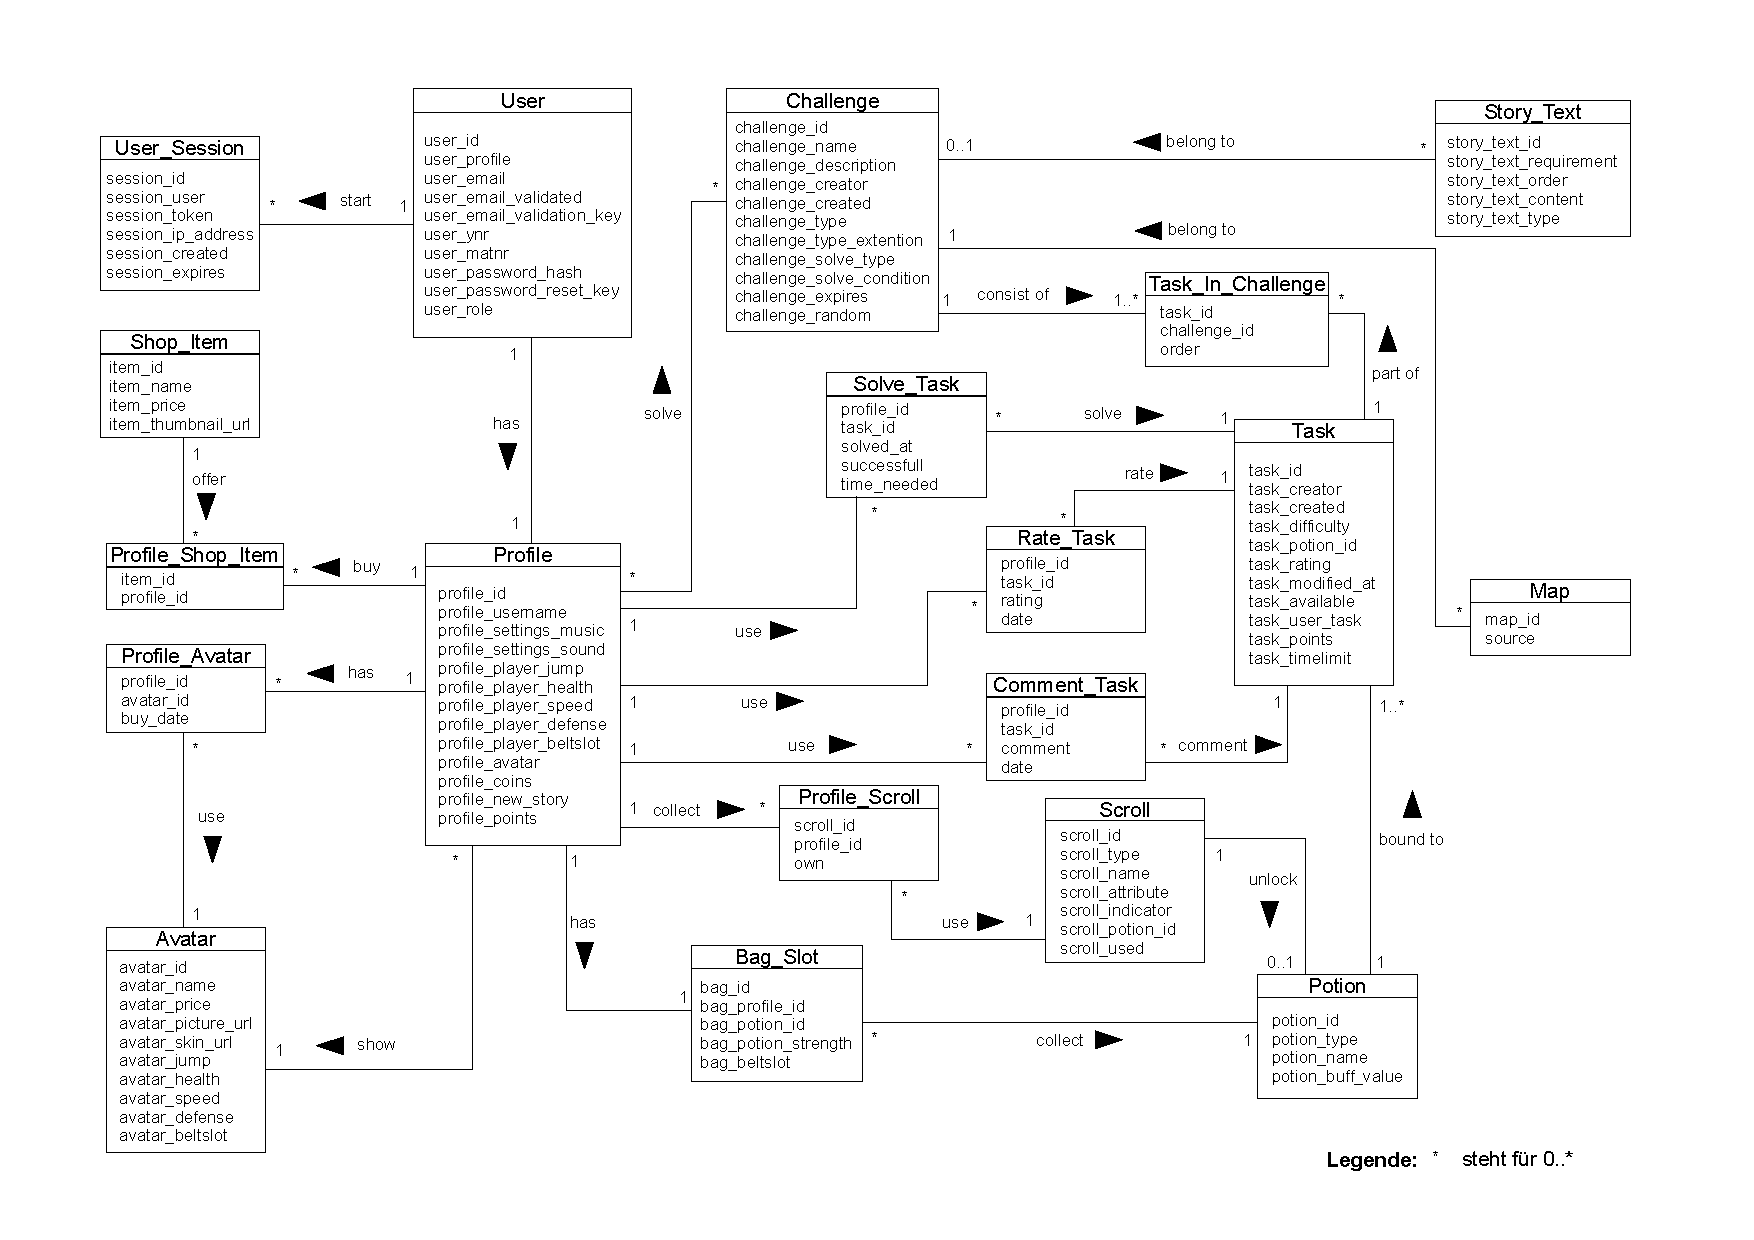
\includegraphics[width=1.0\textwidth]{figures/KlassenDiagrammTE.pdf}
\caption{Klassendiagramm zum SQL-Alchemist}
\label{datenmodell}
\end{figure}
\newpage
\newpage

